\scanpage{69}
exacte
\[
0\mathbin{-}\delta'\mathbin{-}\delta\mathbin{-}\delta''\mathbin{-}0
\]
et la suite exacte associée
\[
0\mathbin{-}{}_n\delta'\mathbin{-}{}_n\delta\mathbin{-}{}_n\delta''\mathbin{-}\delta'_n\mathbin{-}\delta_n\mathbin{-}\delta''_n.
\]
Reste à prouver : \textcircled{a}) le fait que $\Gamma$ est sans torsion. Mais $\unsure{\Gamma|\Gamma_{\mathrm{tors}}}=\mathbf Z/d\mathbf Z$, où $d$ est le pgcd des $d_i$, $X_0=\sum d_iD_i$, \& $X_{0\mathrm{red}}=\sum\unsure{D_i}$. \deleted{On voit que si $\exists$ sur $X$ un cycle \unsure{un cycle} de degré 1} si on a un pt fermé $x$ de $X_\eta$, son adhérence \inserted{\unsure{schématique dans} $X$} est un sous-schéma \inserted{fermé $Z$} \deleted{plat} de $X$, plat et fini sur $S$, \deleted{qui est} dont le degré sur $S$ est aussi égal à la multiplicité d'intersection \inserted{$Z.X_0$} sur $X$, qui est $\sum d_iZ.D_i$, donc multiple de $d$. Donc si $d'\deleted{\unsure{d}}$ est le pgcd des degrés des 0-cycles sur $X_\eta$, on a $d\mid d'$. Comme $d'=1$, on a $d=1$.
\margin{\uline{donner lemme} (ici \unsure{est} $X$ régulier, \unsure{substantiel})}

\textcircled{b}) $\Gamma\longrightarrow\operatorname{NS}(X_0)$ est \uline{injectif}.
\margin{\uline{donner \unsure{corollaire}} \uline{th.}}
[\unsure{Si est} $R$ son noyau, \inserted{qui est $\mathbf Z$ libre et t.t. \unsure{p. 0}}, \deleted{On} a la suite exacte
\[
0\mathbin{-}\mathrm H^1(X,\mu_n)\longrightarrow\mathrm H^1(X_{\bar\eta},\mu_n)^I\longrightarrow\unsure{{}_n\Gamma_n|\Gamma_n}\mathbin{-}\operatorname{NS}(X_0)_n
\]
d'où, par passage à la limite sur les puissances d'un $\ell$
\[
0\mathbin{-}\mathrm H^1(X,\mathbf Z_\ell(1))\mathbin{-}\mathrm H^1(X_{\bar\eta},\mathbf Z_\ell(1))^I\longrightarrow\unsure{\widehat{T}_\ell(\Gamma)\otimes\mathbf Z_\ell|\Gamma\otimes\mathbf Z_\ell}\mathbin{-}\unsure{\widehat{T}_\ell(\operatorname{NS}(X_0))\otimes\mathbf Z_\ell|\operatorname{NS}(X_0)\otimes\mathbf Z_\ell}
\]
i.e. on trouve, comme $\deleted{\unsure{T_\ell R\simeq}}R\otimes\mathbf Z_\ell\simeq\operatorname{Ker}(\Gamma\otimes\mathbf Z_\ell\mathbin{-}\operatorname{NS}(X_0)\otimes\mathbf Z_\ell)$
\deleted{$\unsure{T_\ell R}$}\quad\unsure{$\rho$}
\[
0\mathbin{-}\mathrm H^1(X,\mathbf Z_\ell(1))\mathbin{-}\mathrm H^1(X_{\bar\eta},\mathbf Z_\ell(1))^I\mathbin{-}R\otimes\mathbf Z_\ell\mathbin{-}0.
\]
Donc notre assertion équivaut à dire que l'on a la formule des cycles invariants ; \deleted{\unsure{comme}} il suffit de la prouver à torsion près.]
\margin{[\quad] en remarque après le cor.}

\deleted{L'idée est de se ramener au cas où $X$ est de dim relative un. Dans ce cas, on sait que $\unsure{\Gamma}$ est nul ($\unsure{D_i.D_j}$, c'est le fait que \unsure{son associé} matrice \inserted{d'intersection} est de rang $\unsure{r-1}$, où $r$ est le nb de composantes $D_i$).}
\figure{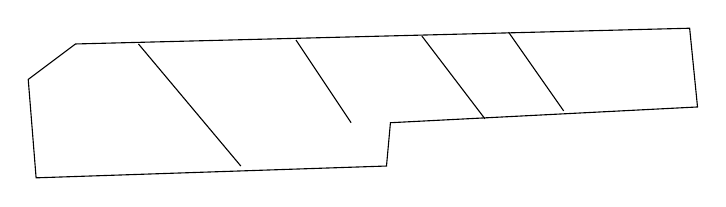
\begin{tikzpicture}[x=1cm,y=1cm]
\draw (0,1.4)--(.6,1.85)--(8.4,2.05)--(8.5,1.05)--(4.6,.85)--(4.55,.3)--(.1,.15)--(0,1.4);
\draw (1.4,1.85)--(2.7,.3);\draw (3.4,1.9)--(4.1,.85);\draw (5.0,1.95)--(5.8,.9);\draw (6.1,2)--(6.8,1);
\end{tikzpicture}}
Or c'est fait par Raynaud dans sa note : spécialisation des foncteurs de Picard, \uline{th. 3} --- dans version sans \deleted{\unsure{dans}} hyp. projective.
\margin{\unsure{donner dém. directe, en cas de dim. rel. 1}}
\deleted{[\unsure{Le fait le plus simple que} $\unsure{R^I}$ \unsure{est} \illegible{3} \unsure{se ramène} \illegible{5}]}
\figure{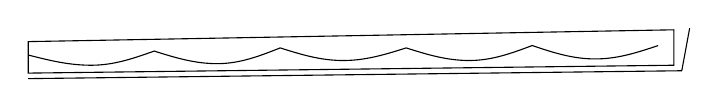
\begin{tikzpicture}[x=1cm,y=1cm]
\draw (0,0)--(8.2,.1)--(8.2,.55)--(0,.4)--cycle;
\draw (0,.23) sin (.8,.1) cos (1.6,.28) sin (2.4,.12) cos (3.2,.32) sin (4,.16) cos (4.8,.32) sin (5.6,.16) cos (6.4,.35) sin (7.2,.18) cos (8,.35);
\draw (0,-.07)--(8.3,.03);\draw (8.3,.03)--(8.4,.57);
\end{tikzpicture}}
\margin{68}
